% vim: set textwidth=78 autoindent:

\section{Integración de GRASS GIS}\label{sec:grass}\index{GRASS}

% when the revision of a section has been finalized, 
% comment out the following line:
%\updatedisclaimer

El complemento de GRASS proporciona acceso a los conjuntos de datos y las funcionalidades de GRASS GIS~\cite{GRASSweb}.
Esto incluye la visualización de capas ráster y vectoriales, digitalización de capas vectoriales, edición de atributos
de vectoriales, crear nuevas capas vectoriales y análisis de datos 2D y 3D de GRASS con más de 300 módulos de GRASS.

En esta sección presentaremos las funcionalidades del complemento y daremos algunos ejemplos sobre la organización 
y trabajo con datos de GRASS. A continuación se proporcionan las principales funciones con el menú de la barra de 
herramientas, cuando inicia el complemento de GRASS, como se describe en la Sección~\ref{sec:starting_grass}:
 
\begin{itemize}
\item \toolbtntwo{grass_open_mapset}{Abrir directorio de mapas}
\item \toolbtntwo{grass_new_mapset}{Nuevo directorio de mapas}
\item \toolbtntwo{grass_close_mapset}{Cerrar directorio de mapas}
\item \toolbtntwo{grass_add_vector}{Añadir capa vectorial de GRASS}
\item \toolbtntwo{grass_add_raster}{Añadir capa ráster de GRASS}
\item \toolbtntwo{grass_new_vector_layer}{Crear nuevo vectorial de GRASS}
\item \toolbtntwo{grass_edit}{Editar capa vectorial de GRASS}
\item \toolbtntwo{grass_tools}{Abrir herramientas de GRASS}
%\item \toolbtntwo{grass_shell}{Open GRASS Shell}
\item \toolbtntwo{grass_region}{Visualizar la región actual de GRASS} 
\item \toolbtntwo{grass_region_edit}{Editar la región actual de GRASS}
\end{itemize}

\subsection{Iniciar el complemento de GRASS}\label{sec:starting_grass}
\index{GRASS!starting QGIS}

Para usar las funciones de GRASS y/o visualizar capas vectoriales o ráster de GRASS en QGIS, debe seleccionar y cargar 
el complemento de GRASS con el administrador de complementos. 
A continuacion pulse el menú 
\mainmenuopt{Complementos} > \mainmenuopt{Administrar complementos}, 
seleccione \dropmenuopt{GRASS} y pulse \button{Aceptar}. 

Ahora puede comenzar a cargar capas ráster y vectoriales desde una  
\filename{LOCALIZACIÓN} existente de 
GRASS (ver Sección \ref{sec:load_grassdata}). O puede crear una \filename{LOCALIZACIÓN} nueva con QGIS (ver Sección \ref{sec:create_loc}) 
e importar algunos datos ráster y vectoriales (ver Sección \ref{sec:import_loc_data}) 
para análisis posteriores con la
caja de herramientas de GRASS (ver Sección \ref{subsec:grass_toolbox}).

\subsection{Cargar capas ráster y vectoriales de GRASS}\label{sec:load_grassdata}\index{GRASS!loading data}

Con el complemento de GRASS, puede cargar capas vectoriales o ráster usando los botones adecuados de la barra de herramientas. 
Como ejemplo usaremos el conjunto de datos de QGIS de alaska
(ver Sección \ref{label_sampledata}), que incluye una pequeña \filename{LOCALIZACIÓN} de ejemplo con 3 capas vectoriales y 1 mapa ráster de elevación.

\begin{enumerate}
  \item Cree una carpeta nueva \filename{grassdata}, descargue el conjunto de datos de QGIS de alaska \filename{qgis\_sample\_data.zip} desde
  \url{http://download.osgeo.org/qgis/data/} y descomprima el archivo en
  \filename{grassdata}. 
  \item Inicie QGIS.
  \item Si no la ha hecho ya en una sesión anterior de QGIS, cargue el complemento de GRASS pinchando en \mainmenuopt{Complementos} > \mainmenuopt{Administrar complementos} y
  seleccionando \dropmenuopt{GRASS}. Aparecerá la barra de herramientas de GRASS en el menú de barras de herramientas.
  \item En la barra de herramientas de GRASS, pulse el icono \toolbtntwo{grass_open_mapset}{Abrir directorio de mapas} para iniciar el asistente  \filename{DIRECTORIO DE MAPAS}.
  \item Para \filename{Gisdbase} explore y seleccione o introduzca la ruta a la carpeta recién creada \filename{grassdata}.
  \item Ahora debería poder seleccionar la \filename{LOCALIZACIÓN alaska}
  y el DIRECTORIO DE MAPAS \filename{demo}. 
  \item Pulse \button{Aceptar}. Note como algunas de las herramientas de la barra de herramientas de GRASS que estaban desactivadas ahora están activadas.
  \item Pulse en \toolbtntwo{grass_add_raster}{Añadir capa ráster de GRASS}, seleccione el mapa llamado \filename{gtopo30} y pulse \button{Aceptar}. Se visualizará la capa de elevaciones.
  \item Pulse en \toolbtntwo{grass_add_vector}{Añadir capa vectorial de GRASS},
  seleccione el mapa \filename{alaska} y pulse \button{Aceptar}. La capa con el contorno de Alaska se superpondrá sobre el mapa gtopo30. Ahora puede adaptar las propiedades de la capa como se describe en el capítulo \ref{sec:vectorprops}, por ejemplo, cambiar la opacidad o el color de relleno o de línea exterior.
  \item Cargue también las otras dos capas vectoriales \filename{rivers} y
  \filename{airports} y adapte sus propiedades.
\end{enumerate}

Como puede ver, es muy sencillo cargar capas ráster y vectoriales de GRASS en QGIS. Vea las siguientes secciones para editar 
datos de GRASS y crear nuevas \filename{LOCALIZACIONES}. Hay más \filename{LOCALIZACIONES} de 
muestra disponibles en la web de GRASS en \url{http://grass.osgeo.org/download/data.php}.

\begin{Tip}\caption{\textsc{Cargar datos de GRASS}}
\qgistip{Si tiene problemas para cargar datos o QGIS termina de forma anormal, asegúrese de que ha cargado el complemento de GRASS correctamente como se describe en la Sección \ref{sec:starting_grass}.
}
\end{Tip} 

\subsection{LOCALIZACIÓN Y DIRECTORIO DE MAPAS DE GRASS}\label{sec:about_loc}

Los datos de GRASS se guardan en un directorio denominado GISDBASE. Este directorio, 
a menudo llamado \filename{grassdata}, 
se debe crear antes de empezar a trabajar con el complemento de GRASS en QGIS. Dentro de ese directorio, los datos SIG de GRASS están
organizados por proyectos guardados en subdirectorios llamados \filename{LOCALIZACIÓN}. 
Cada \filename{LOCALIZACIÓN} se define 
por su sistema de coordenadas, proyección del mapa y límites geográficos. Cada \filename{LOCALIZACIÓN} puede tener 
varios \filename{DIRECTORIOs DE MAPAS} (subdirectorios de la \filename{LOCALIZACIÓN}) que se usan para subdividir el proyecto 
en diferentes temas, subregiones o entornos de trabajo para distintos miembros de un equipo de trabajo (Neteler \& Mitasova 2008 
\cite{neteler_mitasova08}). Para poder analizar capas vectoriales y ráster con los módulos de GRASS, debe importarlos a una \filename{LOCALIZACIÓN} de GRASS.
\footnote{Esto no es estrictamente cierto - con los módulos de GRASS 
\filename{r.external} y \filename{v.external} puede crear enlaces de sólo lectura a conjuntos de datos externos admitidos por 
GDAL/OGR sin importarlos. Pero como esta no es la forma habitual de empezar a trabajar con GRASS para principiantes, esta funcionalidad no se describirá aquí.}

\begin{figure}[ht]
\begin{center}
\caption{Datos de GRASS en la LOCALIZACIÓN alaska (adaptado de Neteler \& 
Mitasova 2008 \cite{neteler_mitasova08})}\label{fig:grass_location}\smallskip

\includegraphics[clip=true]{grass_location}
\end{center}  
\end{figure}

\subsubsection{Crear una nueva LOCALIZACIÓN de GRASS}\label{sec:create_loc}

Como ejemplo mostramos las instrucciones de cómo se creó la \filename{LOCALIZACIÓN Alaska} de GRASS,
que está en la proyección Albers Equal Area, para el conjunto de datos de muestra de QGIS. Esta
\filename{LOCALIZACIÓN Alaska} de GRASS se usará para todos los ejemplos y ejercicios en los siguientes capítulos
relacionados con GRASS GIS. Es útil descargar e instalar el conjunto de datos en su ordenador \ref{label_sampledata}).

\begin{figure}[ht]
\begin{center}
\caption{Crear una nueva LOCALIZACIÓN de GRASS o un nuevo DIRECTORIO DE MAPAS en QGIS \nixcaption}
\label{fig:create_grass_location}\smallskip
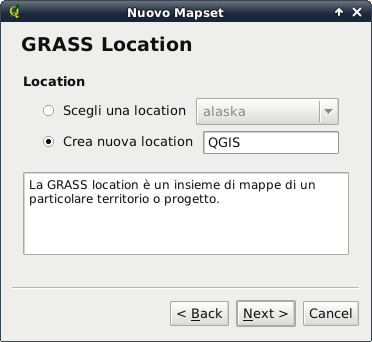
\includegraphics[clip=true, width=10cm]{create_grass_location}
\end{center}  
\end{figure}

\begin{enumerate}
  \item Inicie QGIS y asegúrese de que el complemento de GRASS está cargado.
  \item Visualice el archivo shape \filename{alaska.shp} (ver Sección
  \ref{sec:load_shapefile}) del conjunto de datos alaska de QGIS~\ref{label_sampledata}.
  \item En la barra de herramientas de GRASS, pulse en el icono \toolbtntwo{grass_open_mapset}{abrir
    directorio de mapas} para llamar al asistente \filename{DIRECTORIO DE MAPAS}.
  \item Seleccione una carpeta de base de datos de GRASS (GISDBASE) existente 
  \filename{grassdata} o cree una para la nueva \filename{LOCALIZACIÓN} usando un administrador de archivos 
  de su ordenador. Pulse luego \button{Siguiente}. 
  \item Podemos usar el asistente para crear un nuevo \filename{DIRECTORIO DE MAPAS} dentro de una 
   \filename{LOCALIZACIÓN} existente (ver Sección~\ref{sec:add_mapset}) o para crear 
  una nueva \filename{LOCALIZACIÓN} todo junto. Marque el botón circular
  \radiobuttonon{Crear nueva localización} (ver Imagen \ref{fig:create_grass_location}).
  \item Introduzca un nombre para la \filename{LOCALIZACIÓN} - nosotros usamos alaska y pulse 
  \button{Siguiente} 
  \item Defina la proyección pulsando el botón circular
  \radiobuttonon{Proyección} para activar la lista de proyecciones.
  \item Estamos usando la proyección Albers Equal Area Alaska (pies). Como sabemos que está representada por el EPSG ID 2964, lo introducimos 
  en la casilla de búsqueda. (Nota: Si quiere repetir este proceso para otra 
  \filename{LOCALIZACIÓN} y proyección y no ha memorizado el EPSG ID, 
  pulse en el icono
  \toolbtntwo{mIconProjectionEnabled}{proyector} en la esquina inferior derecha de la barra de estado (ver Sección \ref{label_projstart})).
  \item Pulse \button{Encontrar} para seleccionar la proyección.
  \item Pulse \button{Siguiente} 
  \item TPara definir la región predeterminada, tenemos que introducir los límites de la \filename{LOCALIZACIÓN} en dirección Norte, Sur, Este y Oeste. 
  Aquí simplemente pulsaremos el botón \button{Establecer la extensión actual de QGIS}, para aplicar la extensión de la  
  capa cargada \filename{alaska.shp} como extensión de la región predeterminada de GRASS.
  \item Pulse \button{Siguiente} 
  \item Tambión tenemos que definir un \filename{DIRECTORIO DE MAPAS} dentro de nuestra nueva 
  \filename{LOCALIZACIÓN}. Póngale el nombre que prefiera - nosotros usamos demo.
  \footnote{Cuando se crea una nueva \filename{LOCALIZACIÓN}, GRASS automáticamente 
  crea un \filename{DIRECTORIO DE MAPAS} especial llamado \filename{PERMANENT} diseñado para 
  guardar los datos básicos del proyecto, su extensión espacial predeterminada y 
  la deficición del sistema de coordenadas (Neteler \& Mitasova 2008 
  \cite{neteler_mitasova08}).}
  \item Compruebe el resumen para asegurarse que es correcto y pulse
  \button{Terminar} 
  \item Se creará la nueva \filename{LOCALIZACIÓN alaska} y dos \filename{DIRECTORIO DE MAPAS demo}
  y \filename{PERMANENT}. El conjunto de trabajo abierto actual es el
  \filename{DIRECTORIO DE MAPAS demo}, como lo ha definido.
  \item Vea como algunas de las herramientas de la barra de herramientas de GRASS que estaban desactivadas ahora están activadas.
\end{enumerate}

Si le parecieron muchos pasos, ésto no es tan malo y sí una forma muy rápida de crear una \filename{LOCALIZACIÓN}. La \filename{LOCALIZACIÓN alaska} ahora está lista para importar datos (ver Sección \ref{sec:import_loc_data}).
También puede usar los datos vectoriales y ráster ya existentes en la \filename{LOCALIZACIÓN alaska} de muestra incluida en el conjunto de datos de Alaska de QGIS 
\ref{label_sampledata} e ir a la Sección \ref{label_vectmodel}.

\subsubsection{Añadir un nuevo DIRECTORIO DE MAPAS}\label{sec:add_mapset}

Un usuario sólo tiene permiso de escritura en el \filename{DIRECTORIO DE MAPAS} de GRASS que ha creado. Esto 
significa, además de acceder a su propio \filename{DIRECTORIO DE MAPAS}, cada usuario también puede leer mapas en los 
\filename{DIRECTORIOS DE MAPAS} de otros usuarios, pero sólo puede modificar o eliminar los mapas de su propio 
\filename{DIRECTORIO DE MAPAS}. Todos los \filename{DIRECTORIOS DE MAPAS} incluyen un archivo 
\filename{WIND} que guarda los valores de coordenadas del contorno actual y 
la resolución ráster actualmente seleccionada (Neteler \& Mitasova 2008 
\cite{neteler_mitasova08}, ver Sección \ref{sec:grass_region}). 

\begin{enumerate}
  \item Inicie QGIS y asegúrese de que el complemento de GRASS está cargado.
  \item En la barra de herramientas de GRASS, pulse en el icono 
  \toolbtntwo{grass_new_mapset}{Nuevo directorio de mapas} para lanzar el asistente
  \filename{DIRECTORIO DE MAPAS}.
  \item Seleccione la carpeta de la base de datos de GRASS (GISDBASE) \filename{grassdata} 
  con la \filename{LOCALIZACIÓN alaska}, donde queremos añadir un nuevo 
  \filename{DIRECTORIO DE MAPAS}, llamado test.
  \item Pulse \button{Siguiente}. 
  \item Podemos usar este asistente para crear un nuevo \filename{DIRECTORIO DE MAPAS} dentro de 
  una \filename{LOCALIZACIÓN} existente o crear una nueva \filename{LOCALIZACIÓN} 
  todo a la vez. Pulse el botón circular
  \radiobuttonon{Seleccionar localización} 
  (ver Imagen \ref{fig:create_grass_location}) y pulse \button{Siguiente}.
  \item Introduzca el nombre \filename{text} para el nuevo \filename{DIRECTORIO DE MAPAS}. En la parte de abajo 
  del asistente verá una lista de \filename{DIRECTORIOS DE MAPAS} existente y sus propietarios.
  \item Pulse \button{Siguiente}, Compruebe el resumen para asegurarse de que todo está correcto y pulse \button{Finalizar} 
\end{enumerate}

\subsection{Importar datos a una LOCALIZACIÓN de GRASS}\label{sec:import_loc_data}

Esta Sección da un ejemplo de cómo importar datos ráster y vectoriales a la 
\filename{LOCALIZACIÓN} 
\filename{alaska} de GRASS proporcionada por el conjunto de datos alaska de QGIS. Por lo tanti usaremos un mapa ráster de cobertura
del terreno \filename{landcover.img} y un archivo vectorial GML \filename{lakes.gml} del conjunto de datos alaska de QGIS \ref{label_sampledata}.

\begin{enumerate}
  \item Inicie QGIS y asegúrese de que el complemento de GRASS está cargado.
  \item En la barra de herramientas de GRASS, pulse en el icono 
  \toolbtntwo{grass_open_mapset}{Abrir DIRECTORIO DE MAPAS} para lanzar el asistente
  \filename{DIRECTORIO DE MAPAS}.
  \item Seleccione como base de datos de GRASS la carpeta \filename{grassdata} del conjunto 
  de datos alaska de QGIS, la \filename{LOCALIZACIÓN alaska}, y el \filename{DIRECTORIO DE MAPAS} 
  \filename{demo} y pulse \button{Aceptar}.
  \item Ahora pulse el icono \toolbtntwo{grass_tools}{Abrir herramientas de GRASS}. Aparecerá la caja de herramientas de 
  GRASS (ver Sección \ref{subsec:grass_toolbox}).
  \item Para importar el mapa ráster \filename{landcover.img}, pulse en el módulo 
  \filename{r.in.gdal} en la pestaña 
  \tab{Árbol de módulos}. Este módulo de GRASS le permite importar archivos ráster admitidos por GDAL a una 
  \filename{LOCALIZACIÓN} de GRASS. Aparecerá el diálogo del módulo para \filename{r.in.gdal}.
  \item Navegue a la carpeta \filename{raster} en el conjunto de datos alaska de QGIS y seleccione el archivo \filename{landcover.img}.
  \item Como nombre del ráster de salid defina \filename{landcover\_grass} y pulse 
  \button{Ejecutar}. En la pestaña \tab{Salida} se ve la orden de GRASS que se está ejecutando actualmente 
  \filename{r.in.gdal -o input=/path/to/landcover.img 
  output=landcover\_grass}.
  \item Cuando diga \textbf{Terminado con éxito} pulse \button{Ver salida}. 
  La capa ráster \filename{landcover\_grass} ahora está importada a GRASS y se visualizará en el lienzo de QGIS.
  \item Para importar el archivo GML vectorial \filename{lakes.gml}, pulse el módulo 
  \filename{v.in.ogr} en la pestaña \tab{Árbol de módulos}. Este módulo de GRASS permite importar archivos vectoriales admitidos 
  por OGR a una \filename{LOCALIZACIÓN} de GRASS. Aparecerá el dialogo del módulo para
  \filename{v.in.ogr}.
  \item Navegue a la carpeta \filename{gml} del conjunto de datos alaske de QGIS y seleccione el archivo \filename{lakes.gml} como archivo OGR.
  \item Como nombre del vectorial de salida defina \filename{lakes\_grass} y pulse 
  \button{Ejecutar}. No tiene que preocuparse 
  de las otras opciones en este ejemplo. En la pestaña \tab{Salida} se ve la instrucción de GRASS que se está ejecutando
  \filename{v.in.ogr -o dsn=/path/to/lakes.gml output=lakes\_grass}.
  \item Cuando diga \textbf{Terminado con éxito} pulse \button{Ver salida}. 
  La capa vectorial \filename{lakes\_grass} ahora está importa a GRASS y se visualizará en el lienzo de QGIS.
\end{enumerate}


\subsection{El modelo de datos vectoriales de GRASS}\label{label_vectmodel}\index{GRASS!vector data
model}

Es importante entender el modelo de datos vectoriales de GRASS antes de digitalizar.\index{GRASS!digitizing} En general, GRASS usa un modelo vectorial topológico.\index{GRASS!topology} Esto significa que las áreas no se representan como polígonos cerrados, sino por uno o más contornos. Esto significa que las áreas no se representan como polígonos cerrados, sino por uno o más contornos.
Los contornos deben estar conectados sin saltos. Un área es identificada (etiquetada) por los centroides del área.

Además de contornos y centroides, un mapa vectorial puede contener puntos y líneas. Todos estos elementos geométricos 
pueden estar mezclados en un vectorial y se representarán en diferentes «capas» dentro de un mapa vectorial de GRASS.
Así, en GRASS una capa no es un mapa vectorial o ráster, sino un nivel dentro de un mapa vectorial. Es importante distinguir esto claramente.
\footnote{Aunque es posible mezclar elementos de distinta geometría, no es habitual e incluso en GRASS sólo se usa en casos especiales
tales como el análisis de redes vectoriales. Normalmente es preferible guardar elementos de distinta geometría en diferentes capas.}

Es posible guardar más «capas» en un conjunto de datos vectorial. Por ejemplo, se pueden guardar campos, bosques y lagos en un vectorial.
Los bosques y lagos adyacentes pueden compartir el mismo contorno, pero tiene tablas de atributos separadas. También es posible
adjuntar atributos a los contornos. Por ejemplo, el contorno entre lago y bosque es una carretera, por lo que puede tener una tabla de atributos diferente.
 
La «capa» de los objetos espaciales se define por la «capa» dentro de GRASS. «Capa» es un número que define si hay más de 
una capa dentro del conjunto de datos, por ejemplo, si la geometría es bosque o lago. De momento, puede ser sólo un número, 
en el futuro GRASS también admitirá nombres como campos en la interfaz de usuario.

Los atributos se pueden guardar dentro de la \filename{LOCALIZACIÓN} de GRASS como DBase o SQLITE3 o en bases de datos externas, por ejemplo PostgreSQL, MySQL, 
Oracle, etc.\index{GRASS!attribute storage}

Los atributos en las tablas de las bases de datos se enlazan a los elementos geométricos usando un valor de «categoría».
\index{GRASS!attribute linkage} La «categoría» (clave, ID) es un entero adjunto a los primitivos de la geometría y se 
usa como el enlace a una columna de la tabla de la base de datos.

\begin{Tip}\caption{\textsc{Aprender el modelo vectorial de GRASS}}
\qgistip{
La mejor forma de aprender el modelo vectorial de GRASS y sus capacidades es descargar uno de los muchos manuales de GRASS, donde se describe el modelo vectorial con más detalle. Vea \url{http://grass.osgeo.org/gdp/manuals.php} para más información, libros y manuales en varios idiomas.
}
\end{Tip} 

\subsection{Crear una nueva capa vectorial de GRASS}\label{sec:creating_new_grass_vectors}\index{GRASS!Creating new vectors|see{editing!creating a new layer}}

Para crear una neuva capa vectorial de GRASS con el complemento de GRASS pulse el icono de la barra de herramientas 
\toolbtntwo{grass_new_vector_layer}{Crear nuevo vectorial de GRAS}. Introduca un nombre en el cuadro de texto y puede comenzar 
a digitalizar puntos, líneas o polígonos, siguiendo el procedimiento descrito en la Sección 
\ref{grass_digitising}. 

En GRASS es posible organizar todo tipo de geometrías (puntos, líneas y áreas) en una capa, porque GRASS usa un modelo
vectorial topológico, así que no necesita seleccionar el tipo de geometría al crear un nuevo vectorial de GRASS. Esto es
diferente de la creación de archivos shape con QGIS, ya que los archivos shape utilizan el modelo vectorial de objetos 
espaciales simples (ver Sección \ref{sec:create shape}).

\begin{Tip}\caption{\textsc{Crear una tabla de atributos para una nueva capa vectorial de GRASS}}
\qgistip{
Si quiere asignar atributos a los objetos espaciales digitalizados de su geometría, asegúrese de crear una tabla de 
atributos con las columnas necesarias antes de empezar a digitalizar (ver Imagen \ref{fig:grass_digitizing_table}).
}
\end{Tip} 

\subsection{Digitalizar y editar una capa vectorial de GRASS}\index{GRASS!digitizing tools}\label{grass_digitising}

Las herramientas de digitalización para las capas vectoriales de GRASS son accesibles usando el icono \toolbtntwo{grass_edit}{Editar capa vectorial de GRASS} 
de la barra de herramientas. Asegúrese de que ha cargado un vectorial de GRASS y que éste es la capa seleccionada en 
la leyenda antes de pulsar la herramienta de edición. La figura \ref{fig:grass_digitizing_category} muestra el diálogo
de edición de GRASS que aparece cuando pulsa en la herramienta de edición. Las herramientas y configuración se describen en las siguientes secciones.

\begin{Tip}\caption{\textsc{Digitalizar polígonos en GRASS}}
\qgistip{
Si quiere crear polígonos en GRASS, primero se digitaliza el contorno del polígono, estableciendo el modo a \usertext{Sin categoría}. 
Luego se añade un centroide (punto de etiqueta) dentro del contorno cerrado, estableciendo el modo a \usertext{Siguiente no usado}. 
La razón es que un modelo vectorial topológico enlaza la información de los atributos de un polígono siempre al centroide
y no al contorno.
}
\end{Tip} 

\minisec{Barra de herramientas}\label{label_grasstoolbar}

En la Figura \ref{fig:grass_digitizing_toolbar} puede ver tlas herramientas de digitalización proporcionadas por el complemento de GRASS. La Tabla \ref{tab:grass_tools}
explica las funcionalidades disponibles.

\begin{figure}[h]
   \begin{center}
   \caption{Barra de herramientas de digitalización de GRASS \nixcaption}\label{fig:grass_digitizing_toolbar} 
   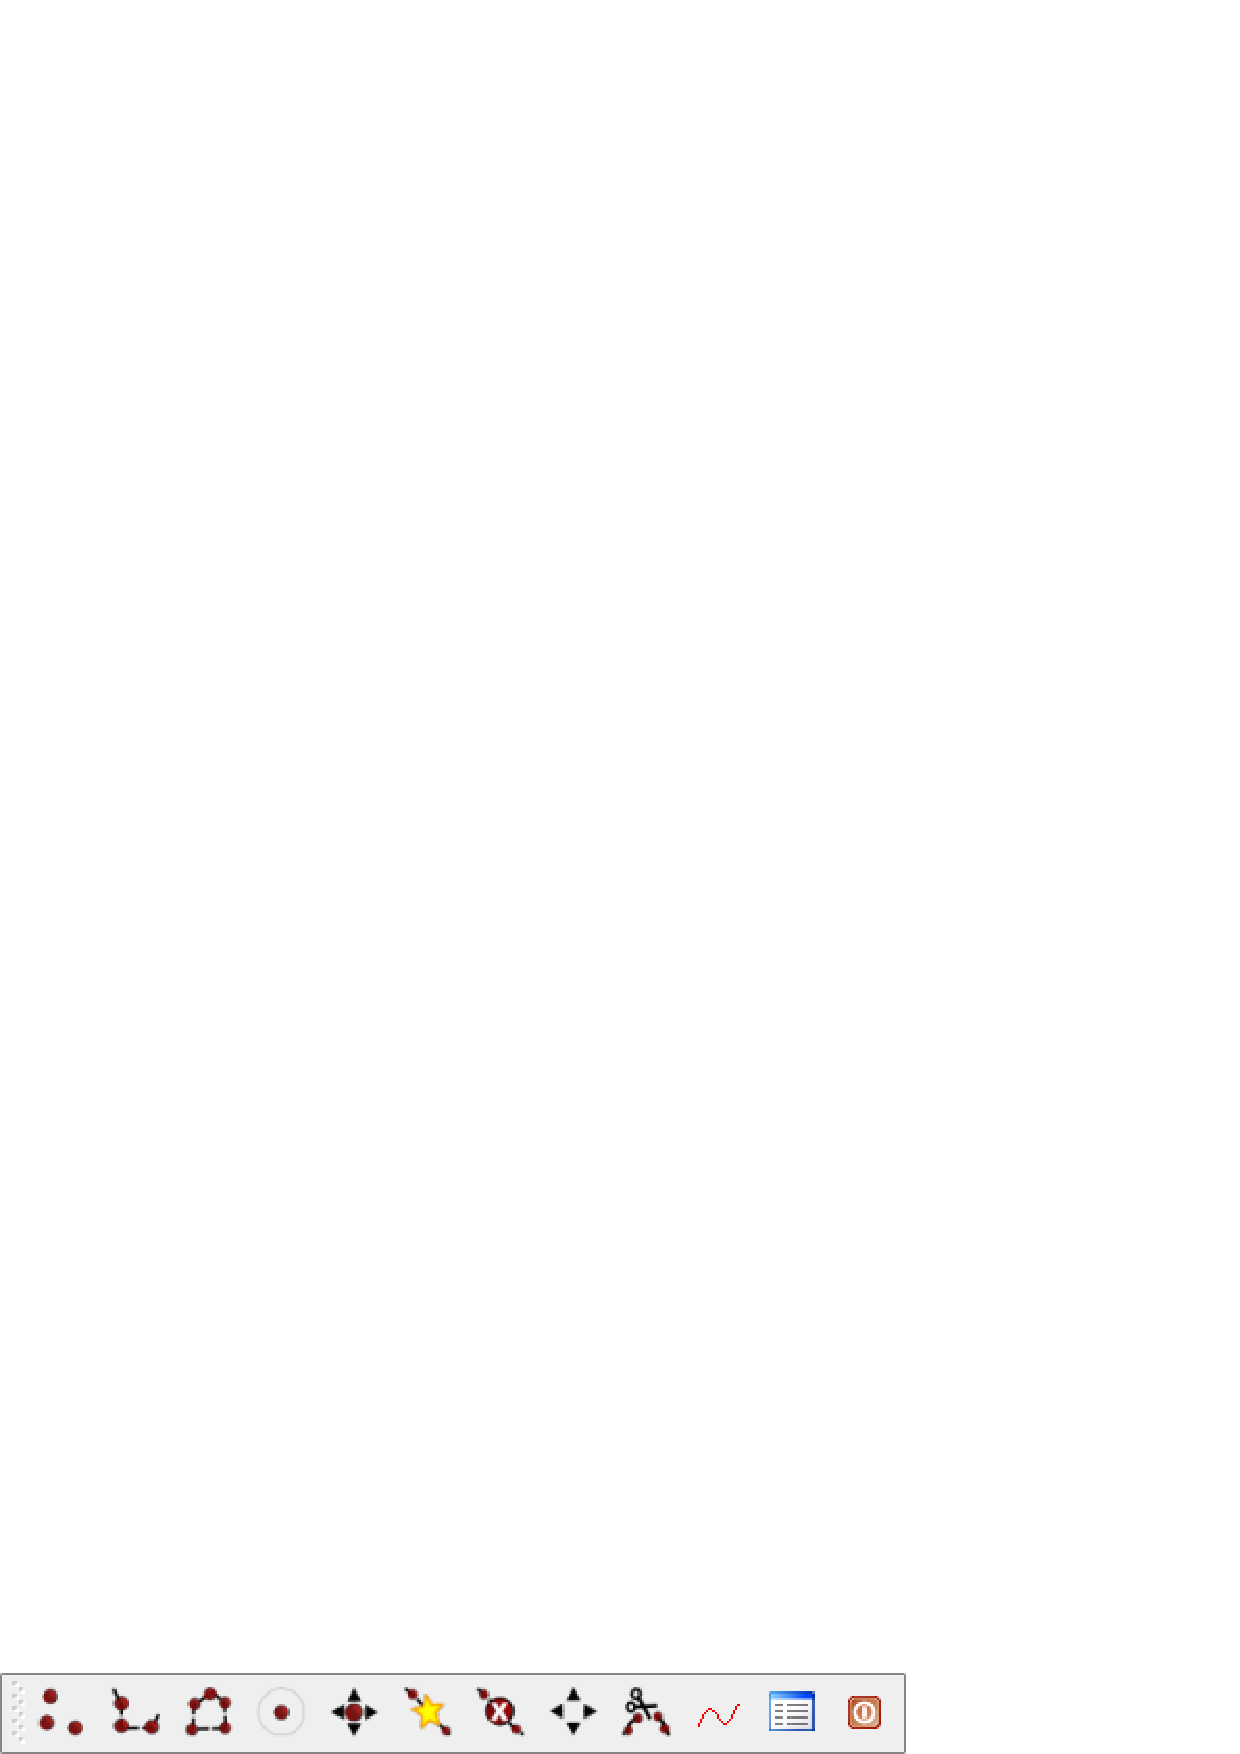
\includegraphics[clip=true,width=12cm]{grass_digitizing_toolbar}
\end{center}  
\end{figure}

\begin{table}[h]\index{GRASS!digitizing tools}
\centering
\caption{Herramientas de digitalización de GRASS}\label{tab:grass_tools}\medskip
 \begin{tabular}{|l|l|p{5in}|}
 \hline \textbf{Icono} & \textbf{Herramienta} & \textbf{Propósito} \\
\hline 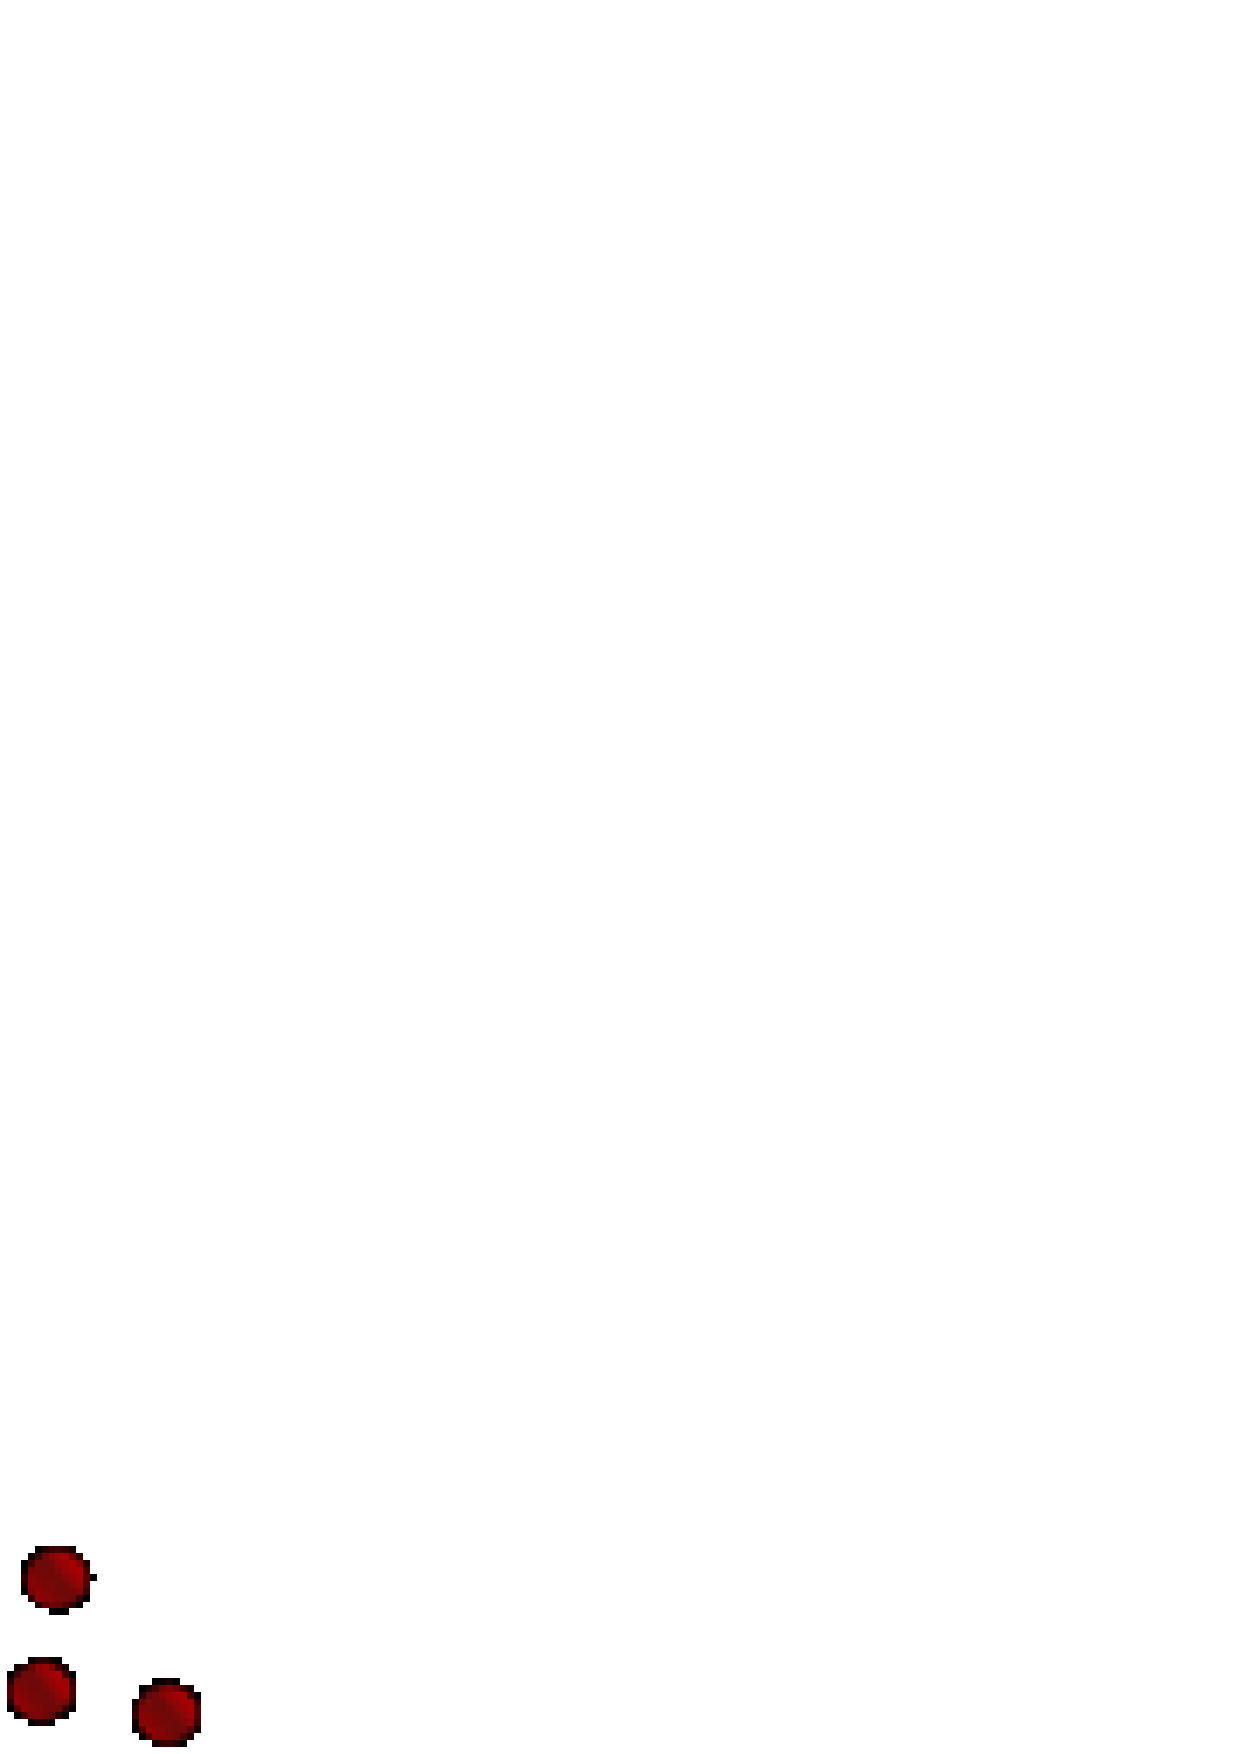
\includegraphics[width=0.7cm]{grass_new_point} & Nuevo punto & Digitalizar un punto nuevo \\
\hline 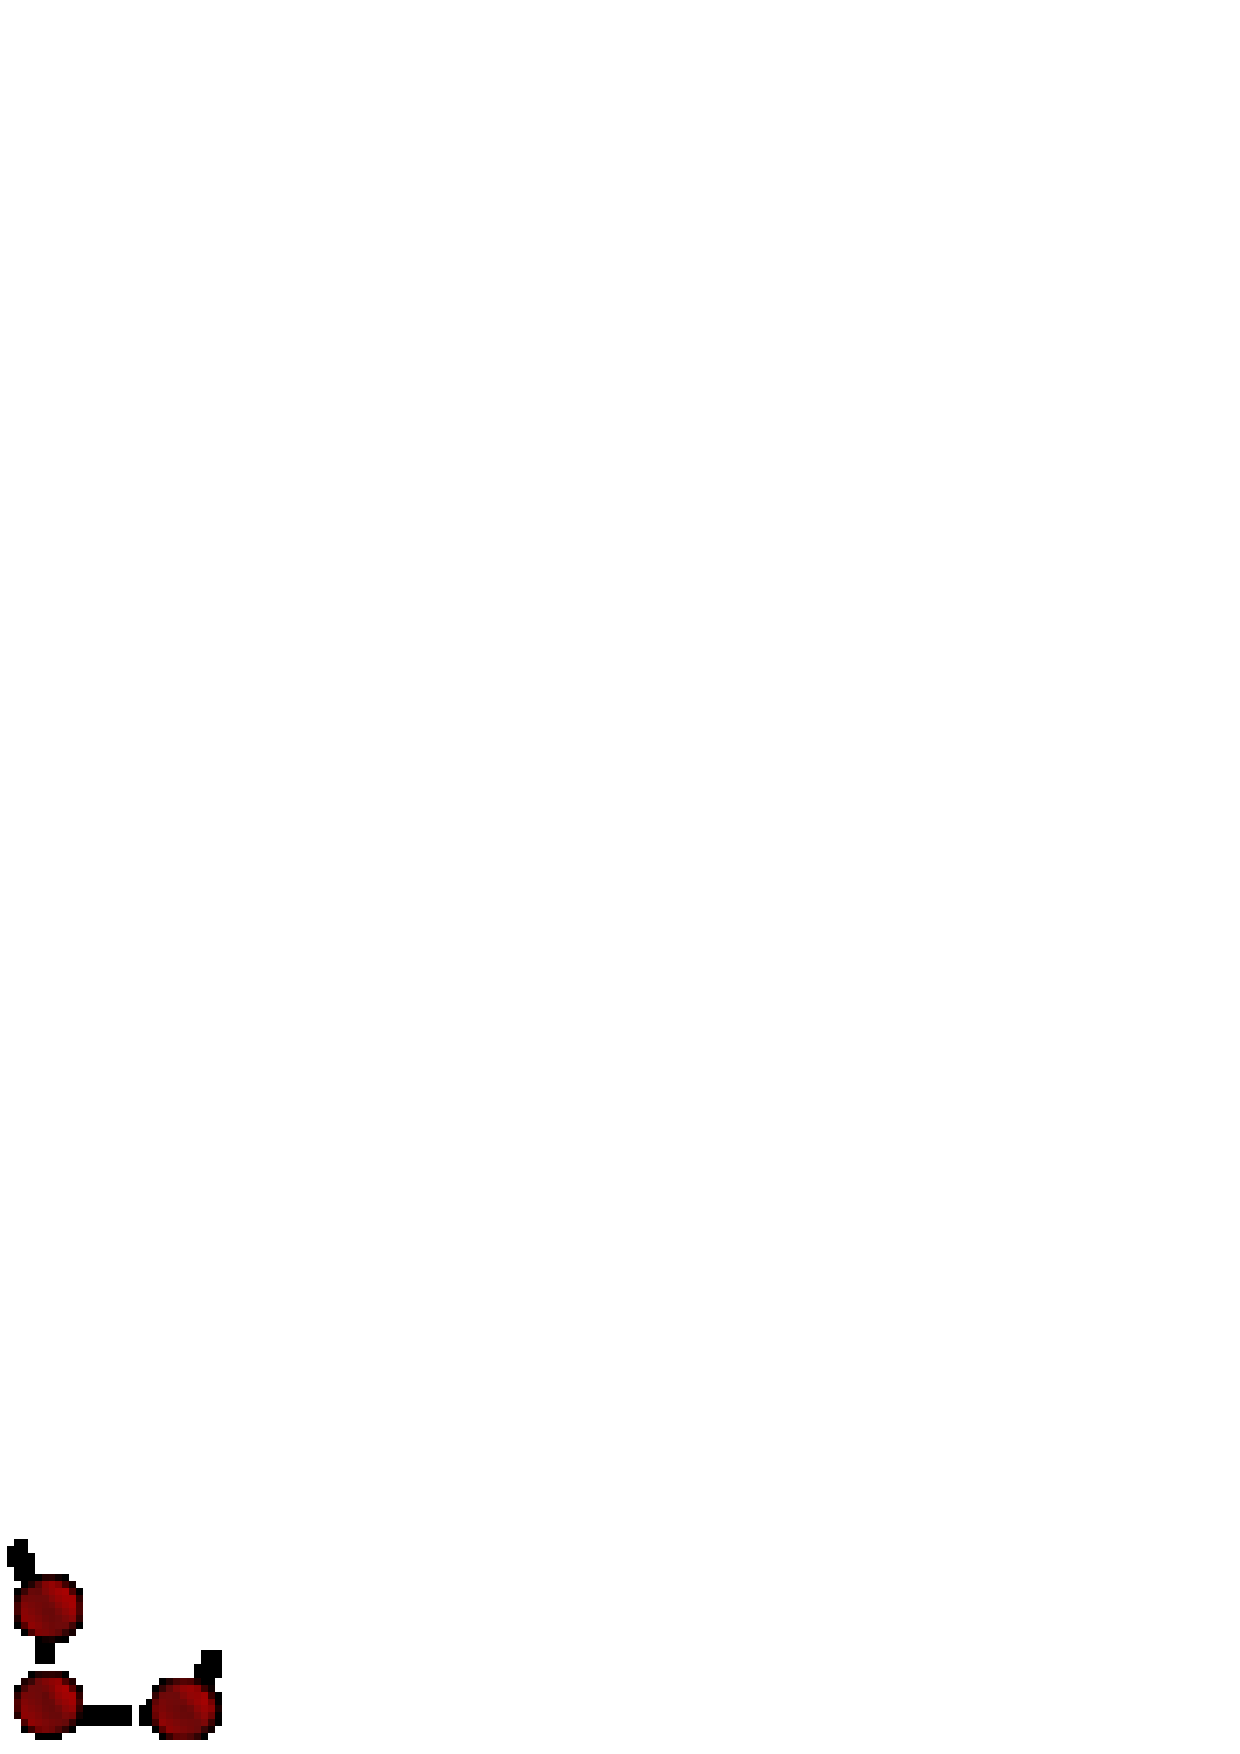
\includegraphics[width=0.7cm]{grass_new_line} & Nueva línea &  Digitalizar una línea nueva (finaliza al seleccionar una herramienta nueva) \\
\hline 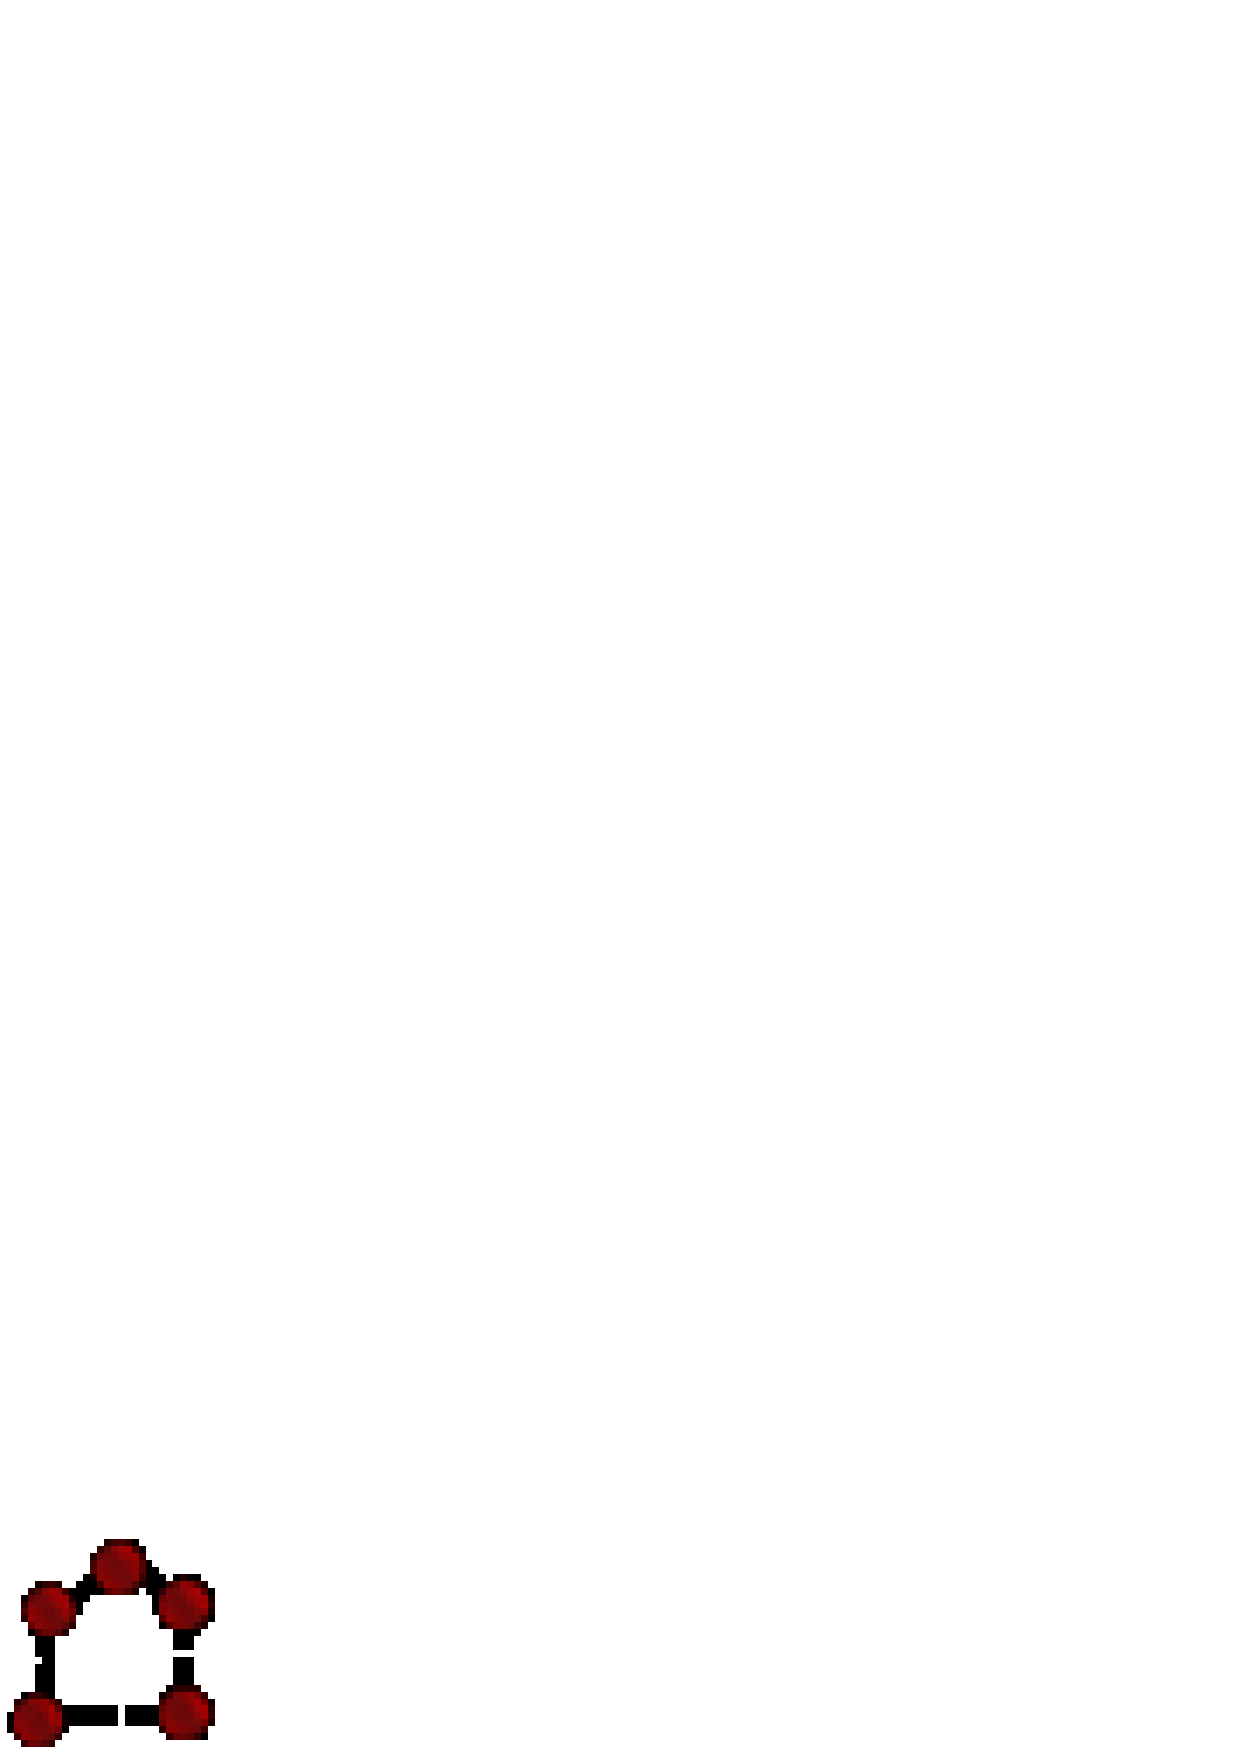
\includegraphics[width=0.7cm]{grass_new_boundary} & Nuevo contorno & Digitalizar un contorno nuevo (finaliza al seleccionar una herramienta nueva)\\
\hline 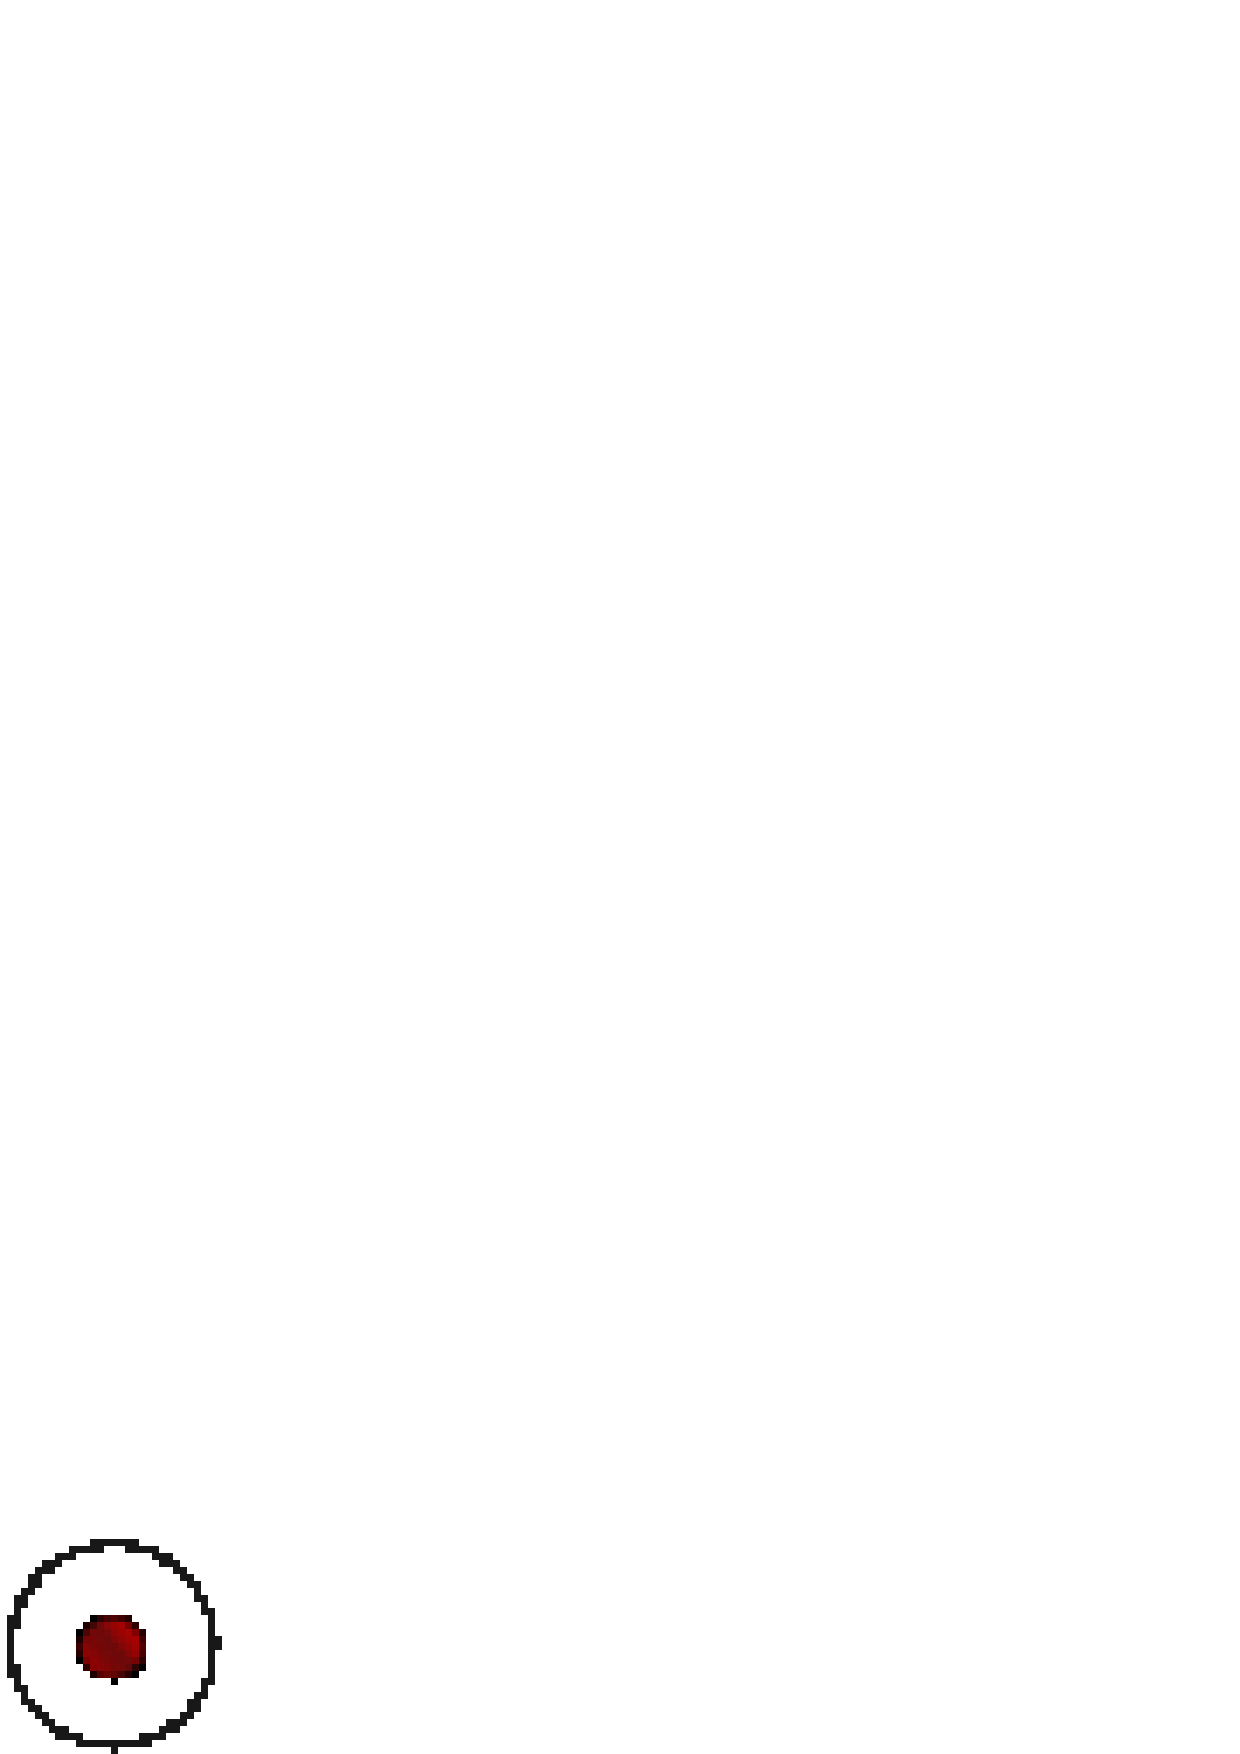
\includegraphics[width=0.7cm]{grass_new_centroid} & Nuevo centroide & Digitalizar un centroide nuevo (etiquetar un área existente)\\
\hline 
\includegraphics[width=0.7cm]{grass_move_vertex} & Mover vértice & Seleccionar un vértice de una línea o contorno existente e identificar una nueva posición\\
\hline 
\includegraphics[width=0.7cm]{grass_add_vertex} & Add vertex & Add a
new vertex to existing line\\
\hline 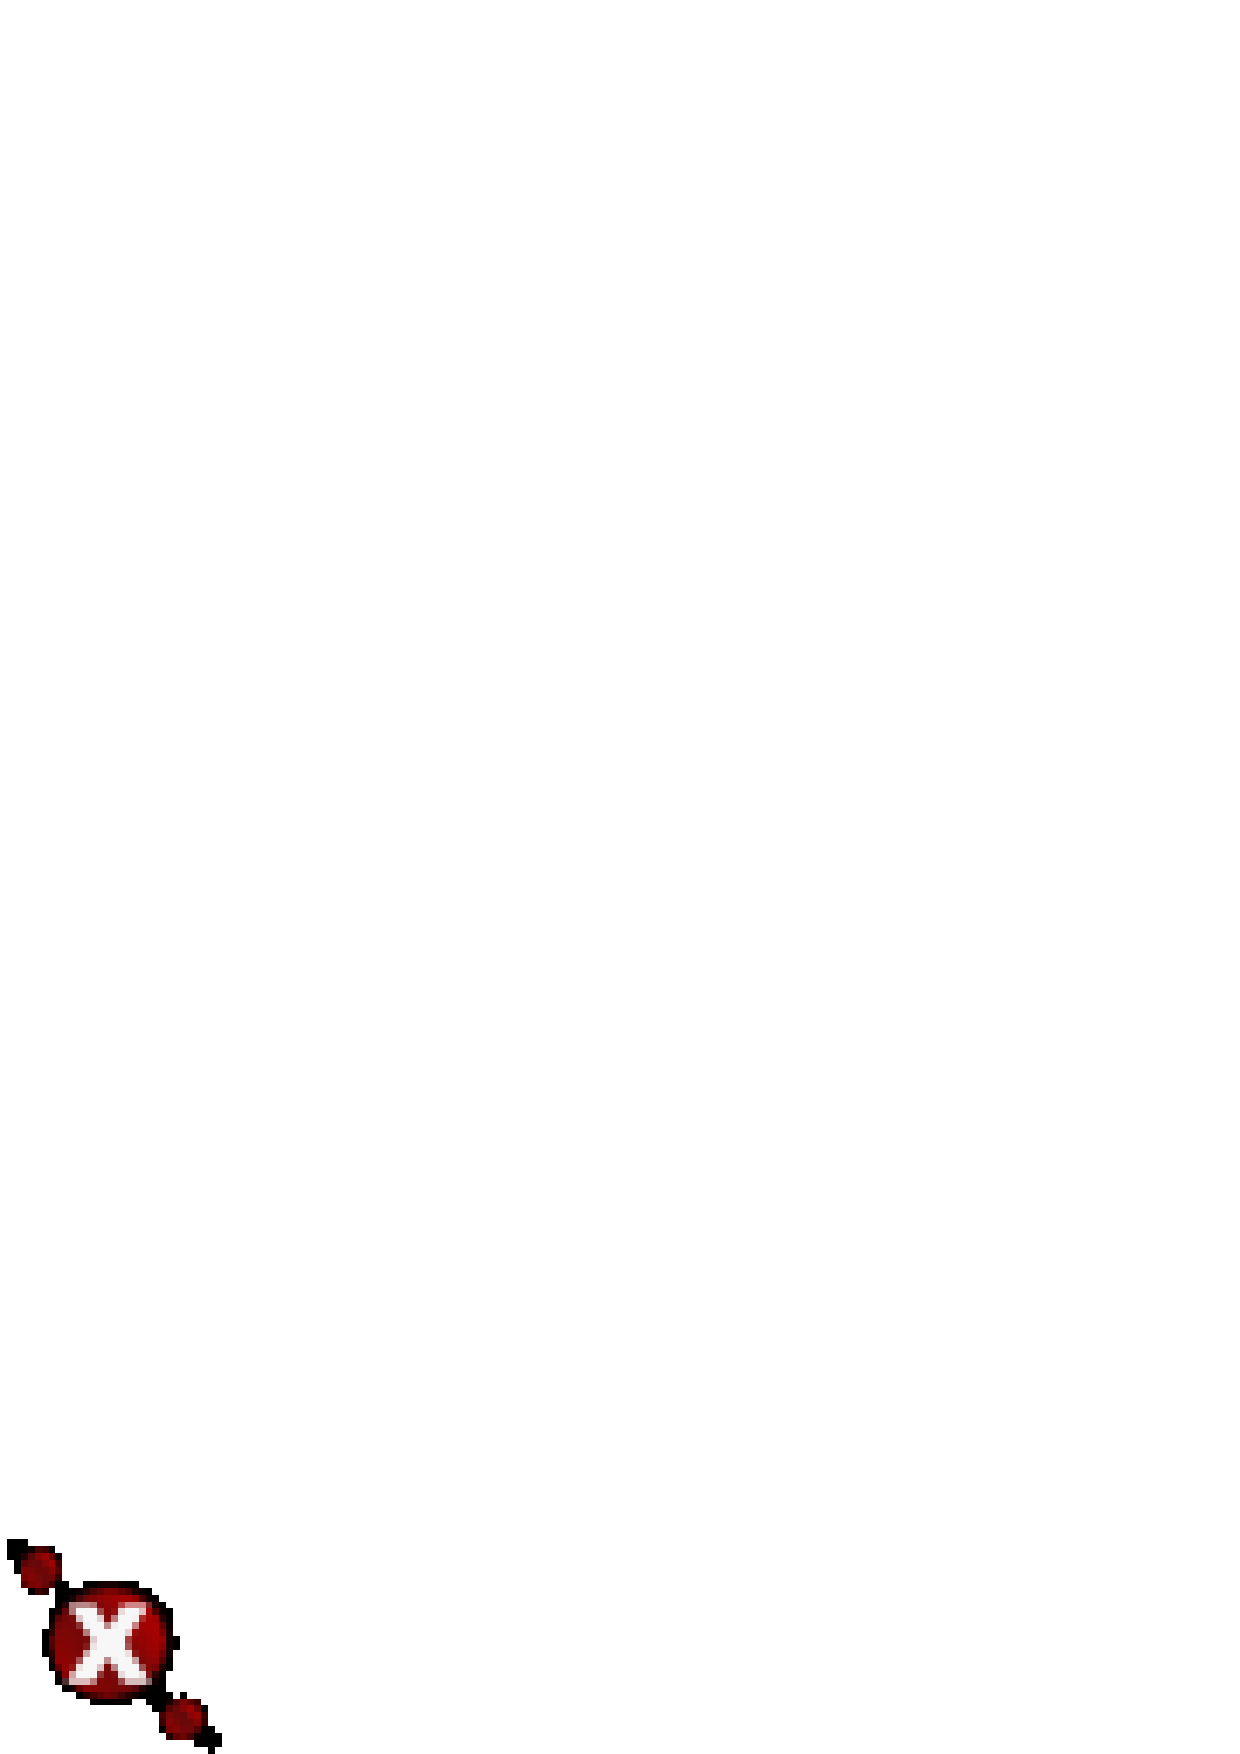
\includegraphics[width=0.7cm]{grass_delete_vertex} & Delete vertex &
Delete vertex from existing line (confirm selected vertex by another click)\\
\hline 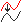
\includegraphics[width=0.7cm]{grass_move_line} & Move element & Move
selected boundary, line, point or centroid and click on new position\\
\hline 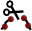
\includegraphics[width=0.7cm]{grass_split_line} & Split line & Split
an existing line to 2 parts\\
\hline 
\includegraphics[width=0.7cm]{grass_delete_line} & Delete element &
Delete existing boundary, line, point or centroid (confirm selected element by
another click)\\
\hline 
\includegraphics[width=0.7cm]{grass_edit_attributes} & Edit attributes
& Edit attributes of selected element (note that one element can represent
more features, see above)\\
\hline 
\includegraphics[width=0.7cm]{grass_close_edit} & Close & Close
session and save current status (rebuilds topology afterwards)\\
\hline
\end{tabular}
\end{table}

\minisec{Category Tab}\index{GRASS!category settings}

The \tab{Category} tab allows you to define the way in which the category 
values will be assigned to a new geometry element.

\begin{figure}[h]
 \begin{center}
  \caption{GRASS Digitizing Category Tab \nixcaption}\label{fig:grass_digitizing_category}
  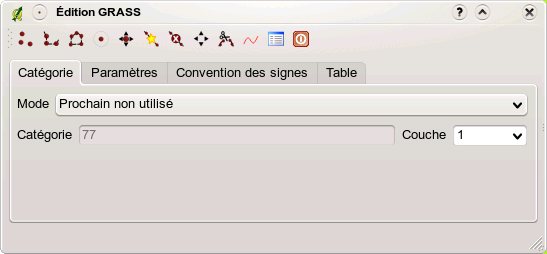
\includegraphics[clip=true,width=10cm]{grass_digitizing_category}
 \end{center}
\end{figure}

\begin{itemize}
\item \textbf{Mode}: what category value shall be applied to new geometry 
elements.
\begin{itemize}
\item Next not used - apply next not yet used category value to geometry
element.
\item Manual entry - manually define the category value for the geometry
element in the 'Category'-entry field.
\item No category - Do not apply a category value to the geometry element.
This is e.g. used for area boundaries, because the category values are
connected via the centroid.
\end{itemize}
\item \textbf{Category} - A number (ID) is attached to each digitized geometry
element. It is used to connect each geometry element with its attributes.
\item \textbf{Field (layer)} - Each geometry element can be connected with
several attribute tables using different GRASS geometry layers. Default layer
number is 1. 
\end{itemize}

\begin{Tip}\caption{\textsc{Creating an additional GRASS 'layer' with QGIS}}
\qgistip{If you would like to add more layers to your dataset, just add a new
number in the 'Field (layer)' entry box and press return. In the Table tab
you can create your new table connected to your new layer.
}
\end{Tip}

\minisec{Settings Tab}\label{label_settingtab}\index{GRASS!snapping
tolerance}

The \tab{Settings} tab allows you to set the snapping in screen pixels. The
threshold defines at what distance new points or line ends are snapped to
existing nodes. This helps to prevent gaps or dangles between boundaries. The
default is set to 10 pixels.

\begin{figure}[h]
 \begin{center}
 \caption{GRASS Digitizing Settings Tab \nixcaption}\label{fig:grass_digitizing_settings}
 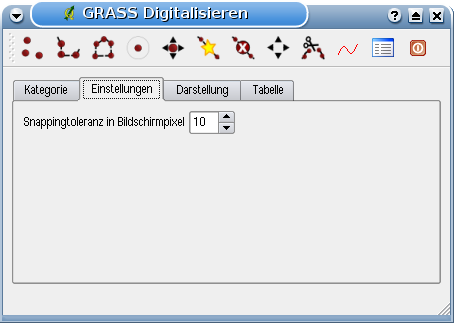
\includegraphics[clip=true,width=8cm]{grass_digitizing_settings}
 \end{center}
\end{figure}

\minisec{Symbology Tab}\index{GRASS!symbology settings}

The \tab{Symbology} tab allows you to view and set symbology and color
settings for various geometry types and their topological status (e.g. closed
/ opened boundary).

\begin{figure}[h]
 \begin{center}
 \caption{GRASS Digitizing Symbolog Tab \nixcaption}\label{fig:grass_digitizing_symbology}
 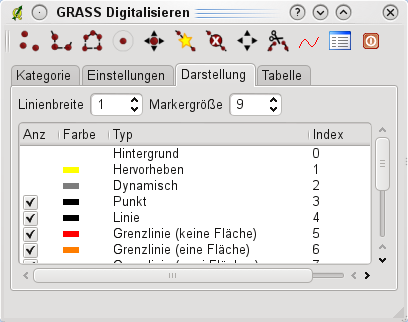
\includegraphics[clip=true,width=8cm]{grass_digitizing_symbology}
 \end{center}
\end{figure}

\minisec{Table Tab} \index{GRASS!table editing}

The \tab{Table} tab provides information about the database table for
a given 'layer'. Here you can add new columns to an existing attribute table,
or create a new database table for a new GRASS vector layer (ver Sección 
\ref{sec:creating_new_grass_vectors}).

\begin{figure}[h]
 \begin{center}
 \caption{GRASS Digitizing Table Tab \nixcaption}\label{fig:grass_digitizing_table}
 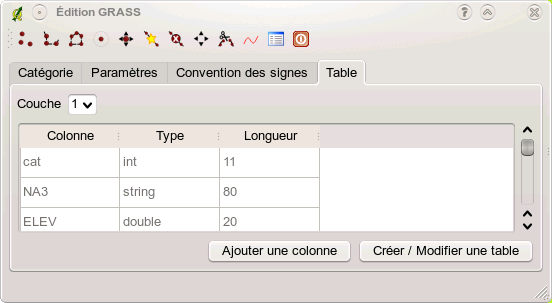
\includegraphics[clip=true,width=10cm]{grass_digitizing_table}
 \end{center}
\end{figure}

\begin{Tip}\caption{\textsc{GRASS Edit Permissions}}\index{GRASS!edit
permissions}
\qgistip{You must be the owner of the GRASS \filename{DIRECTORIO DE MAPAS} you want to 
edit. It is impossible to edit data layers in a \filename{DIRECTORIO DE MAPAS} that is not 
yours, even if you have write permissions.
}
\end{Tip} 

\subsection{The GRASS region tool}\label{sec:grass_region}\index{GRASS!region}

The region definition (setting a spatial working window) in GRASS is important 
for working with raster layers. Vector analysis is per default not limited
to any defined region definitions. All newly-created rasters will have the
spatial extension and resolution of the currently defined GRASS region,
regardless of their original extension and resolution. The current GRASS
region is stored in the \filename{\$LOCATION/\$MAPSET/WIND} file, and it 
defines north, south, east and west bounds, number of columns and rows, 
horizontal and vertical spatial resolution.

It is possible to switch on/off the visualization of the GRASS region in the
QGIS canvas using the \toolbtntwo{grass_region}{Display current GRASS region}
button. \index{GRASS!region!display}.

With the \toolbtntwo{grass_region_edit}{Edit current GRASS region} icon you 
can open a dialog to change the current region and the symbology of the GRASS 
region rectangle in the QGIS canvas. Type in the new region bounds and 
resolution and click \button{OK}. It also allows to select a new region 
interactively with your mouse on the QGIS canvas. Therefore click with the 
left mouse button in the QGIS canvas, open a rectangle, close it using the 
left mouse button again and click \button{OK}.\index{GRASS!region!editing}
The GRASS module \filename{g.region} provide a lot more parameters to define 
an appropriate region extend and resolution for your raster analysis. You can 
use these parameters with the GRASS Toolbox, described in Sección 
\ref{subsec:grass_toolbox}.

\subsection{The GRASS toolbox}\label{subsec:grass_toolbox}\index{GRASS!toolbox}

The \toolbtntwo{grass_tools}{Open GRASS Tools} box provides GRASS module 
functionalities to work with data inside a selected GRASS \filename{LOCALIZACIÓN} 
and \filename{DIRECTORIO DE MAPAS}. To use the GRASS toolbox you need to open a 
\filename{LOCALIZACIÓN} and \filename{DIRECTORIO DE MAPAS} where you have write-permission 
(usually granted, if you created the \filename{DIRECTORIO DE MAPAS}). This is necessary, 
because new raster or vector layers created during analysis need to be written 
to the currently selected \filename{LOCALIZACIÓN} and \filename{DIRECTORIO DE MAPAS}.

\subsubsection{Working with GRASS modules}\index{GRASS!toolbox}

\begin{figure}[h]
\centering
\caption{GRASS Toolbox and searchable Modules List \nixcaption}\label{fig:grass_modules}
   \subfigure[Modules Tree] {\label{subfig:grass_module_tree}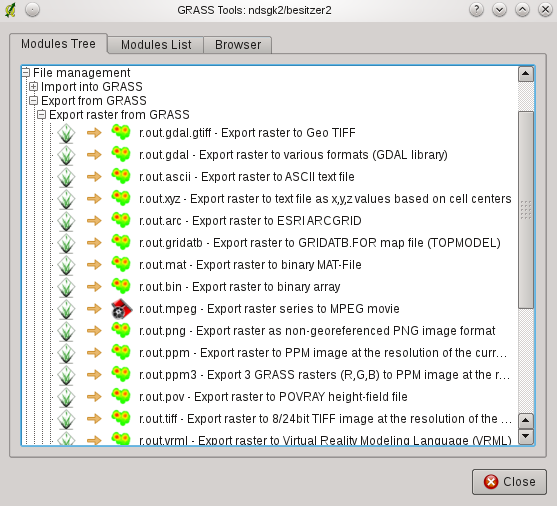
\includegraphics[clip=true, width=0.4\textwidth]{grass_toolbox_moduletree}}\goodgap
   \subfigure[Searchable Modules List] {\label{subfig:grass_module_list}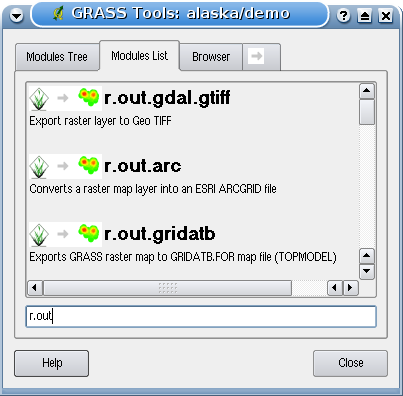
\includegraphics[clip=true, width=0.4\textwidth]{grass_toolbox_modulelist}}
\end{figure}

The GRASS Shell inside the GRASS Toolbox provides access to almost all (more 
than 300) GRASS modules in command line modus. To offer a more user
friendly working environment, about 200 of the available GRASS modules and 
functionalities are also provided by graphical dialogs. These dialogs are 
grouped in thematic blocks, but are searchable as well. You find a complete 
list of GRASS modules available in QGIS version \CURRENT
in appendix \ref{appdx_grass_toolbox_modules}. It is also possible to 
customize the GRASS Toolbox content. It is described in Sección 
\ref{sec:toolbox-customizing}.

As shown in Figure \ref{fig:grass_modules}, you can look for the appropriate 
GRASS module using the thematically grouped \tab{Modules Tree} or the 
searchable \tab{Modules List} tab. 

Clicking on a grapical module icon a new tab will be added to the toolbox 
dialog providing three new sub-tabs \tab{Options}, \tab{Output} and 
\tab{Manual}. In Figure \ref{fig:grass_module_dialog} you see an example 
for the GRASS module \filename{v.buffer}.

\begin{figure}[h]
\centering
\caption{GRASS Toolbox Module Dialogs \nixcaption}\label{fig:grass_module_dialog}
   \subfigure[Module Options] {\label{subfig:grass_module_option}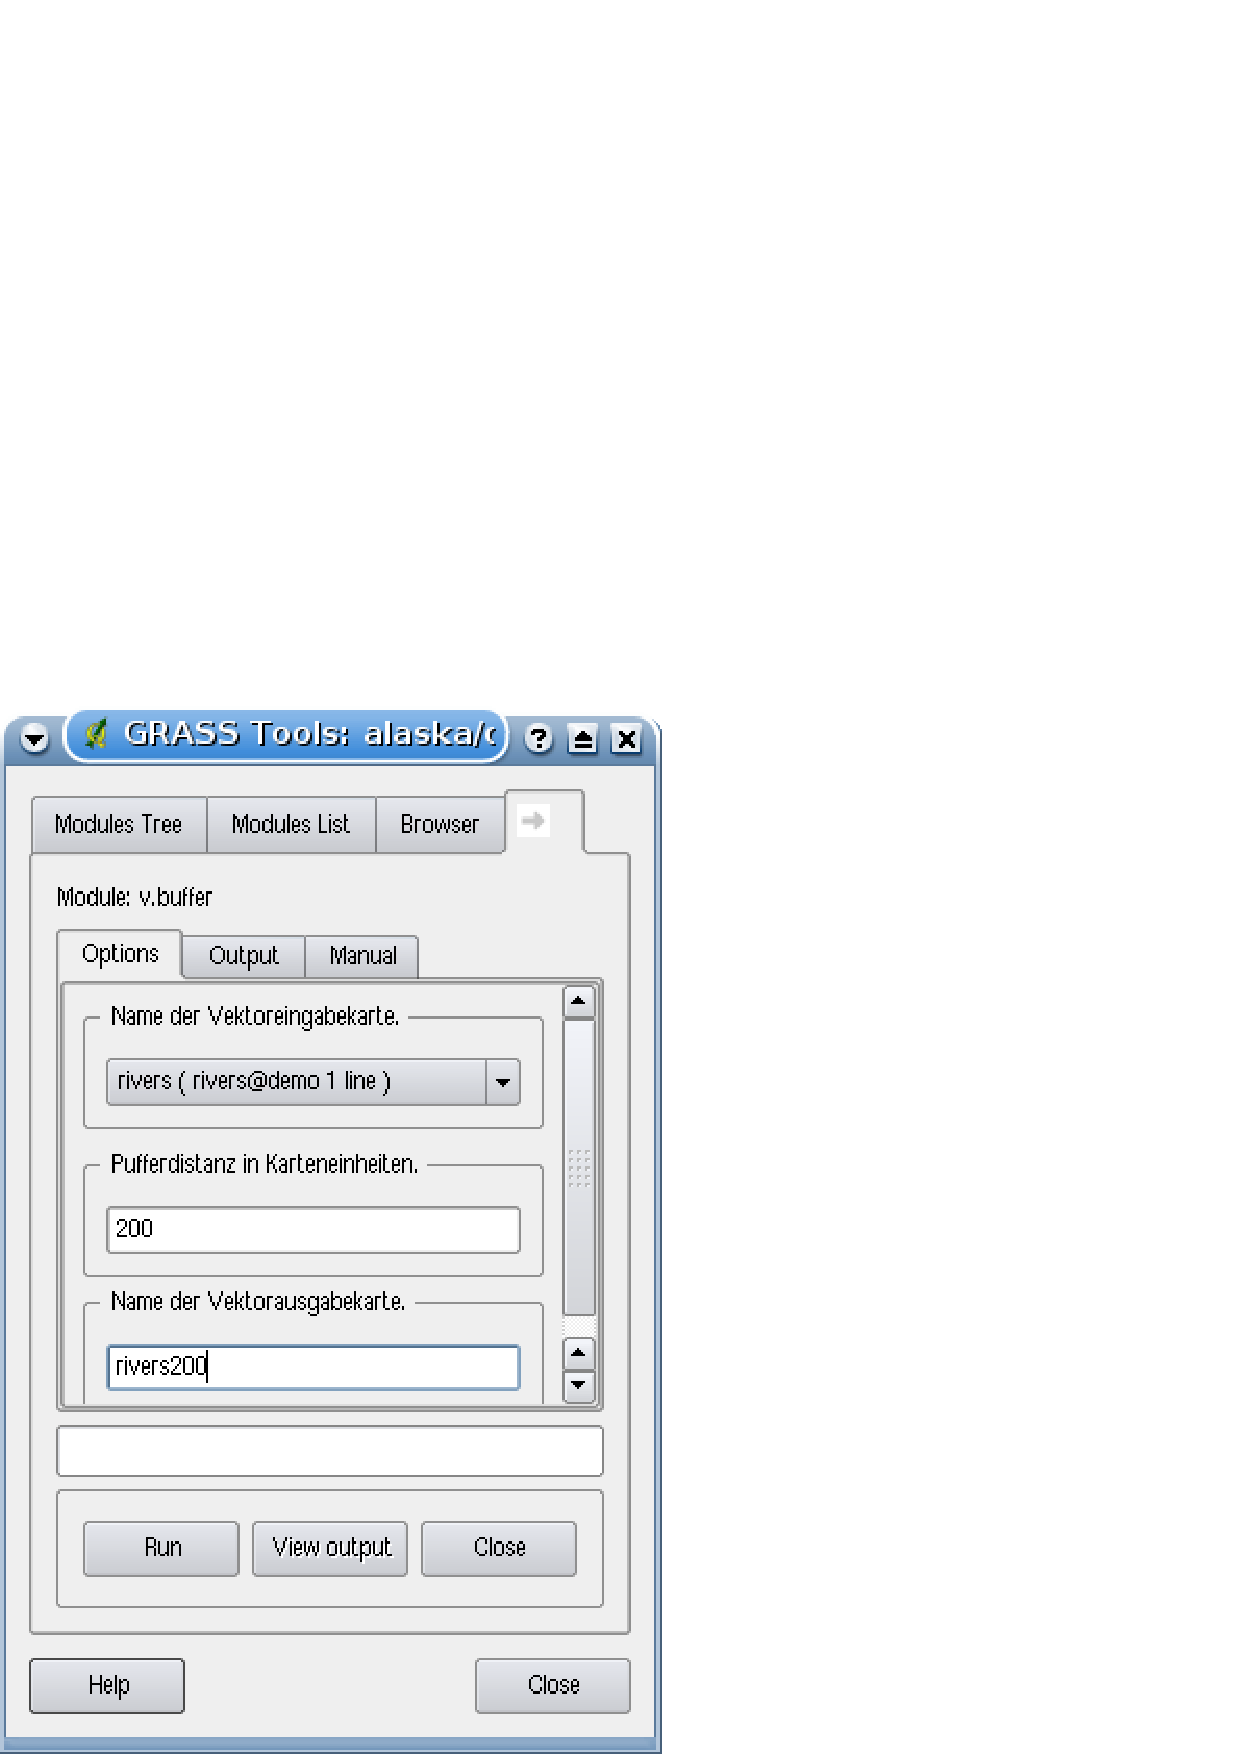
\includegraphics[clip=true, width=0.3\textwidth]{grass_module_option}}\goodgap
   \subfigure[Modules Output] {\label{subfig:grass_module_output}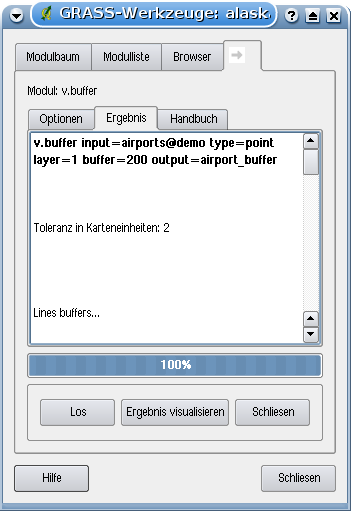
\includegraphics[clip=true, width=0.3\textwidth]{grass_module_output}}\goodgap
   \subfigure[Module Manual] {\label{subfig:grass_module_manual}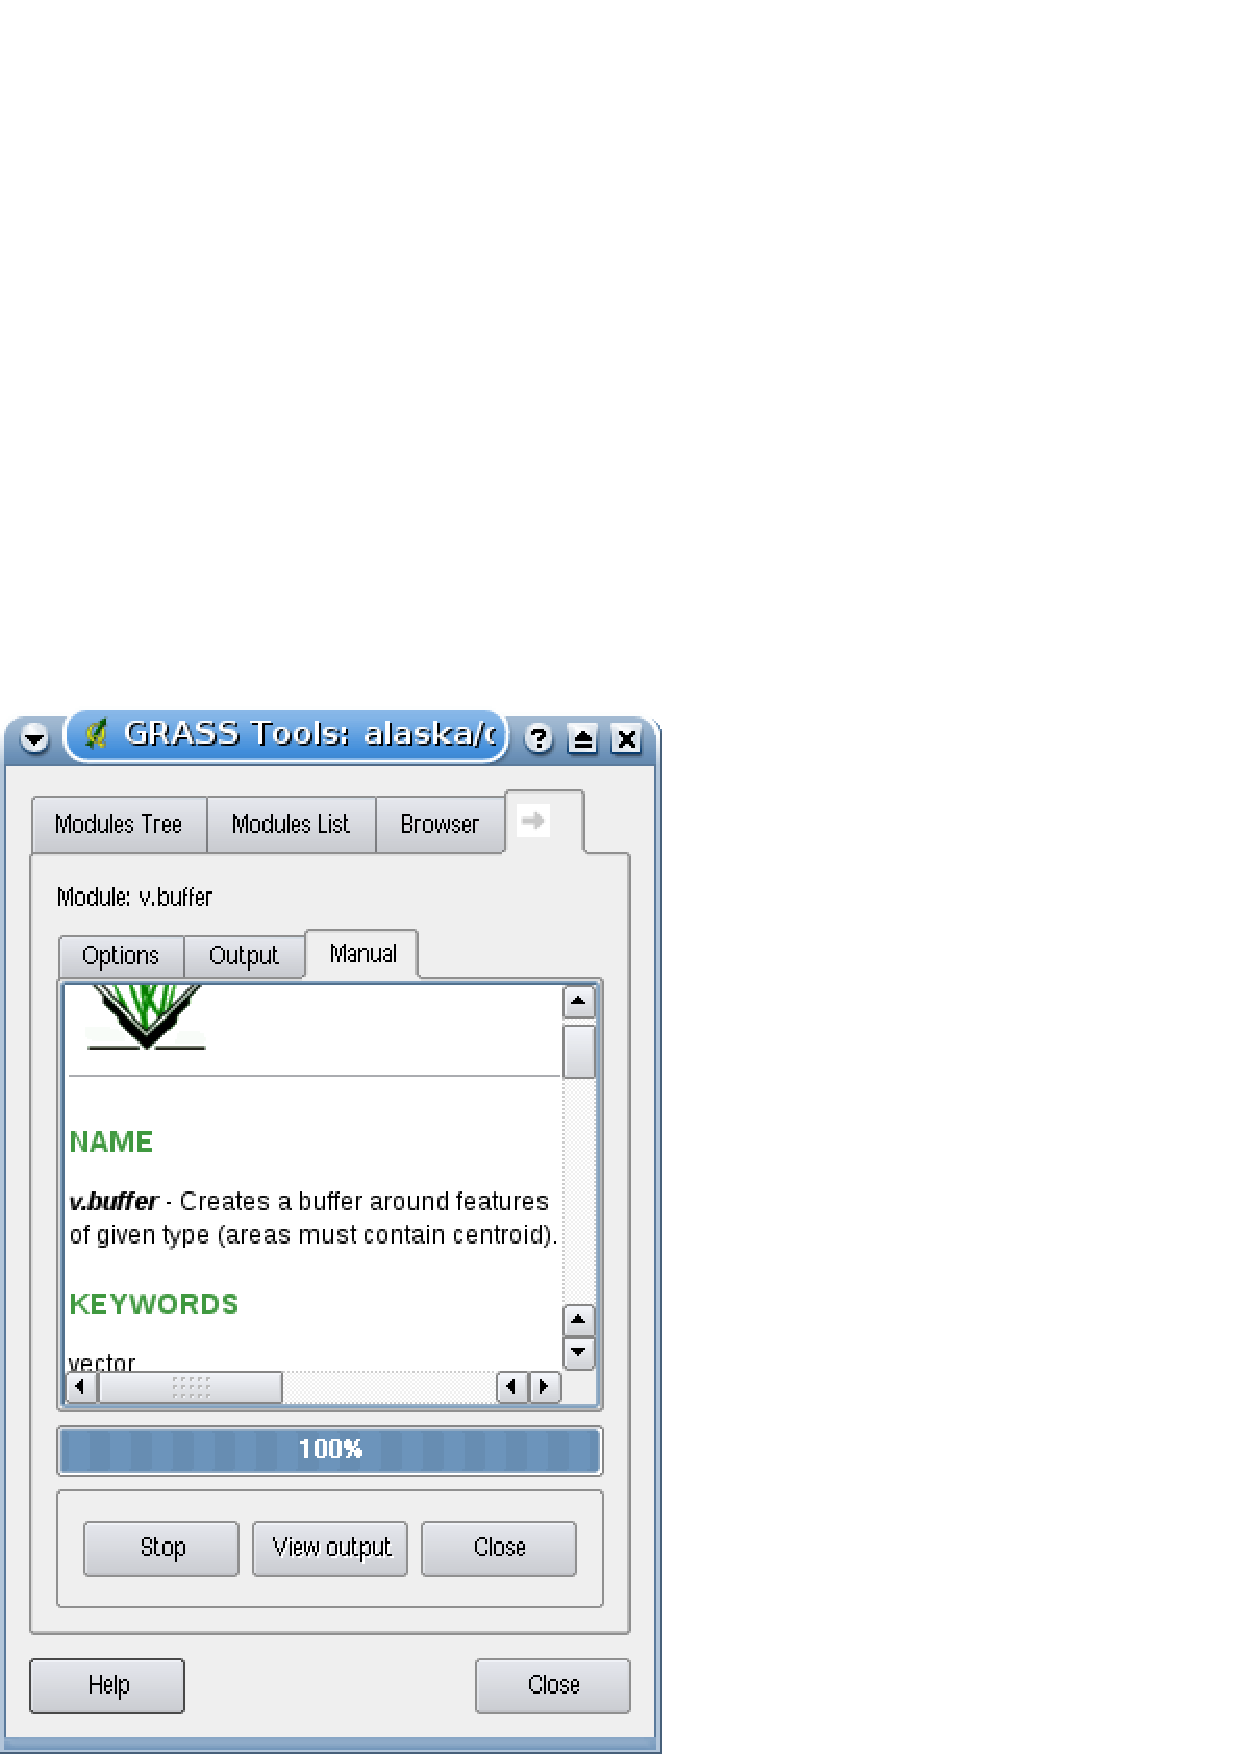
\includegraphics[clip=true, width=0.3\textwidth]{grass_module_manual}}
\end{figure}

\minisec{Options}

The \tab{Options} tab provides a simplified module dialog where you can 
usually select a raster or vector layer visualized in the QGIS canvas and 
enter further module specific parameters to run the module. The provided 
module parameters are often not complete to keep the dialog clear. If you want 
to use further module parameters and flags, you need to start the GRASS Shell 
and run the module in the command line.

\minisec{Output}

The \tab{Output} tab provides information about the output status of the 
module. When you click the \button{Run} button, the module switches to the 
\tab{Output} tab and you see information about the analysis process. If all 
works well, you will finally see a \usertext{Successfully finished} message.

\minisec{Manual}

The \tab{Manual} tab shows the HTML help page of the GRASS module. You can 
use it to check further module parameters and flags or to get a deeper 
knowledge about the purpose of the module. At the end of each module 
manual page you see further links to the \filename{Main Help index}, the 
\filename{Thematic index} and the \filename{Full index}. These links provide 
the same information as if you use the module \filename{g.manual} 

\begin{Tip}\caption{\textsc{Display results immediately}}\index{GRASS!display results}
\qgistip{If you want to display your calculation results immediately in your 
map canvas, you can use the 'View Output' button at the bottom of the 
module tab.
}
\end{Tip} 

\subsubsection{Working with the GRASS LOCALIZACIÓN browser} \index{GRASS!toolbox!Browser}

Another useful feature inside the GRASS Toolbox is the GRASS 
\filename{LOCALIZACIÓN} browser. In Figure~\ref{fig:grass_mapset_browser} you 
can see the current working \filename{LOCALIZACIÓN} with its \filename{MAPSETs}.

In the left browser windows you can browse through all \filename{MAPSETs} 
inside the current \filename{LOCALIZACIÓN}. The right browser window shows some 
meta information for selected raster or vector layers, e.g. resolution, 
bounding box, data source, connected attribute table for vector data and a 
command history.

\begin{figure}[h]
 \begin{center}
 \caption{GRASS LOCALIZACIÓN browser \nixcaption}\label{fig:grass_mapset_browser}
 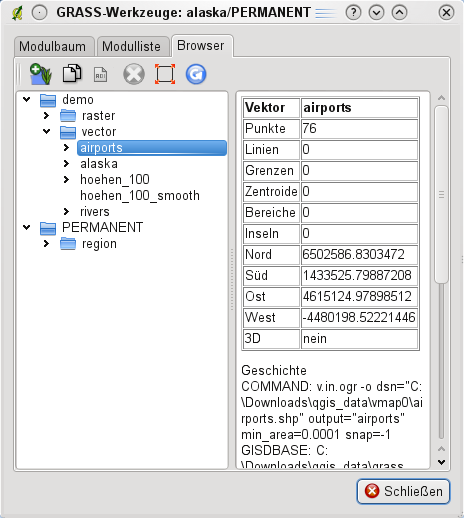
\includegraphics[clip=true,width=10cm]{grass_mapset_browser}
 \end{center}
\end{figure}

The toolbar inside the \tab{Browser} tab offers following tools to manage 
the selected \filename{LOCALIZACIÓN}:

\begin{itemize}
\item \toolboxtwo{grass_add_map}{Add selected map to canvas}
\item \toolboxtwo{grass_copy_map}{Copy selected map}
\item \toolboxtwo{grass_rename_map}{Rename selected map}
\item \toolboxtwo{grass_delete_map}{Delete selected map}
\item \toolboxtwo{grass_set_region}{Set current region to selected map}
\item \toolboxtwo{grass_refresh}{Refresh browser window}
\end{itemize}

The \toolboxtwo{grass_rename_map}{Rename selected map} and 
\toolboxtwo{grass_delete_map}{Delete selected map} only work with maps inside 
your currently selected \filename{DIRECTORIO DE MAPAS}. All other tools also work with 
raster and vector layers in another \filename{DIRECTORIO DE MAPAS}.

\subsubsection{Customizing the GRASS Toolbox} \index{GRASS!toolbox!customize}
\label{sec:toolbox-customizing}

Nearly all GRASS modules can be added to the GRASS toolbox. A XML 
interface is provided to parse the pretty simple XML files which configures 
the modules appearance and parameters inside the toolbox.

A sample XML file for generating the module \usertext{v.buffer} (v.buffer.qgm) 
looks like this:
\begin{verbatim}
<?xml version="1.0" encoding="UTF-8"?>
<!DOCTYPE qgisgrassmodule SYSTEM "http://mrcc.com/qgisgrassmodule.dtd">

<qgisgrassmodule label="Vector buffer" module="v.buffer">
        <option key="input" typeoption="type" layeroption="layer" />
        <option key="buffer"/>
        <option key="output" />
</qgisgrassmodule>
\end{verbatim}

The parser reads this definition and creates a new tab inside the toolbox 
when you select the module. A more detailed description for adding new 
modules, changing the modules group, etc. can be found on the QGIS wiki at \\
\url{http://wiki.qgis.org/qgiswiki/Adding\_New\_Tools\_to\_the\_GRASS\_Toolbox}.

